
\subsubsection{Model Generalization}
\label{sec:randerrC}

Although a key takeaway from Section \ref{sec:randerr} is that the \gls{MLL}
calculations are the most resilient to introduced error in the training set
features for all four prediction categories, there is another aspect of the
algorithm performance not explicitly shown in those plots: generalization.
\Gls{MLL} does not generalize to unseen data; it provides predictions based on
finding the closest training set entry to the test sample.  It (usually)
outperforms the scikit-learn methods in part because the training set is so
large. This is also true for the \textit{k}-nearest neighbor implementations
where $k=1$ (burnup and cooling time, as seen in Table \ref{tbl:exp1hypparam}).

\begin{figure}[!htb]
  \centering
  \begin{subfigure}[b]{0.495\textwidth}
    \centering
    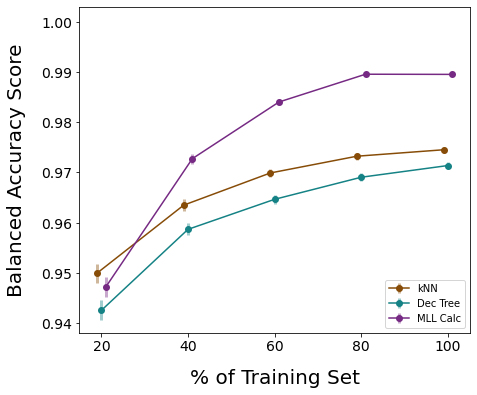
\includegraphics[width=\textwidth]{./chapters/exp1/learncurve_nuc29_err05_BalAcc_rxtr.png}
    \caption{Balanced accuracy of reactor type classification with respect 
             to training set size.}
    \label{fig:learnsA}
  \end{subfigure}
  \hfill
  \begin{subfigure}[b]{0.485\textwidth}
    \centering
    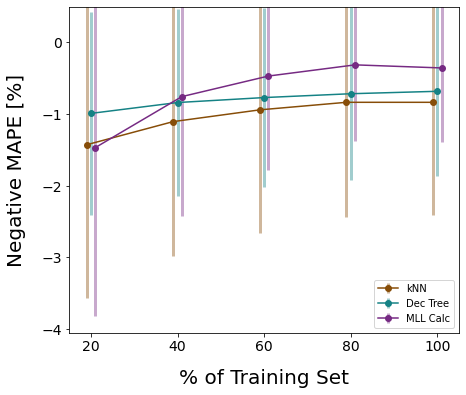
\includegraphics[width=\textwidth]{./chapters/exp1/learncurve_nuc29_err05_MAPE_burn.png}
    \caption{Negative \gls{MAPE} of burnup regression with respect to 
             to training set size.}
    \label{fig:learnsB}
  \end{subfigure}
  \vskip\baselineskip
  \begin{subfigure}[b]{0.48\textwidth}
    \centering
    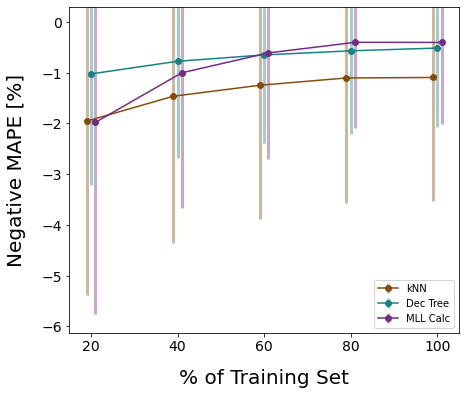
\includegraphics[width=\textwidth]{./chapters/exp1/learncurve_nuc29_err05_MAPE_enri.png}
    \caption{Negative \gls{MAPE} of \gls{U235} enrichment regression with 
             respect to training set size.}
    \label{fig:learnsC}
  \end{subfigure}
  \hfill
  \begin{subfigure}[b]{0.50\textwidth}
    \centering
    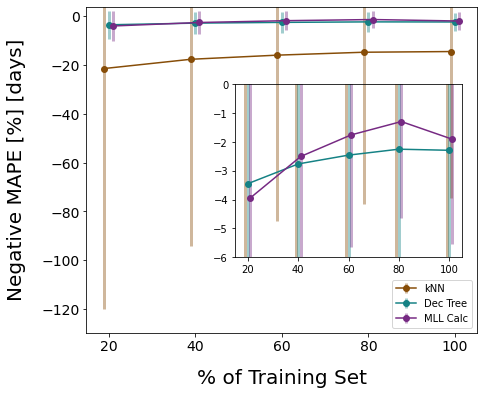
\includegraphics[width=\textwidth]{./chapters/exp1/learncurve_nuc29_err05_MAPE_cool.png}
    \caption{Negative \gls{MAPE} of time since irradiation regression with 
             respect to training set size.}
    \label{fig:learnsD}
  \end{subfigure}
  \caption[Learning curves for all four prediction parameters]
          {Learning curves for reactor type, burnup, enrichment, and time 
           since irradiation with respect to increasing fraction of the 
           training set, for 5\% training set random error.}
  \label{fig:learns}
\end{figure}

One way to show that an algorithm is generalizing well in comparison to others
is to view the shape of its learning curve (introduced in Section
\ref{sec:complexity}): the prediction performance with respect to training set
size.  It is crucial to have the training sets be identical for each algorithm,
so they were created in advance and the learning curves are constructed
manually rather than relying on the scikit-learn method.  Smaller training sets
were created from the original one by taking 80\%, 60\%, 40\%, and 20\% of the
entries. The training sets are all stratified so that the original fractions of
\gls{BWR}, \gls{PWR}, and \gls{PHWR} are retained. They are also built on top
of one another, so the 20\%-size training set is contained within the 40\%-size
set, and so forth.

Learning curves were constructed for all four prediction categories,
demonstrated in Figure \ref{fig:learns}. As in Figures
\ref{fig:randrxtr}--\ref{fig:randcool} , the \textit{y}-axis is always oriented
so that lower is poorer performance and higher is better performance; also, the
error bars reflect a 99\% confidence interval for Figure \ref{fig:learnsA}, and
one standard deviation of the average percentage errors for Figures
\ref{fig:learnsB}--\ref{fig:learnsD}.  These learning curves represent the 5\%
random error case in Figures \ref{fig:randrxtr}--\ref{fig:randcool}, so the
scores/errors in these figures are the data points at the 100\% training set
level in Figure \ref{fig:learns}.  Therefore, the leftmost data in Figure
\ref{fig:learns} will show the \gls{MLL} point being slightly above the
scikit-learn points for the reactor type, burnup, and enrichment predictions,
and the \textit{k}-nearest neighbor point is below the \gls{MLL} and decision
trees points for time since irradiation.  

Figure \ref{fig:learnsA} shows that the balanced accuracy score of reactor type
classification for the \gls{MLL} calculations decreases more at lower training
set size than for the scikit-learn algorithms. Here, the curve crosses below
the \textit{k}-nearest neighbors curve at the lowest training set size of 20\%.
For the burnup \gls{MAPE} in Figure \ref{fig:learnsB} and the enrichment
\gls{MAPE} in Figure \ref{fig:learnsC}, the \gls{MLL} curve crosses below both
of the scikit-learn algorithm curves. This happens between 20\% and 40\%
training set size for burnup, and between 40\% and 60\% training set size for
enrichment.  Lastly, Figure \ref{fig:learnsD} shows a different arrangement,
which is to be expected from the results shown in Figure \ref{fig:randcool},
where the \textit{k}-nearest neighbors performance is significantly worse than
the other two algorithms. Because the \textit{k}-nearest neighbors curve and
error bars are so large, there is an inset showing a closeup of the other two
curves above -6\%.  The decision trees and \gls{MLL} calculations curves now
appear to follow the trend in the burnup and enrichment cases, and the
\gls{MLL} curve crosses under the decision trees curve between 20\% and 40\%
training set size.  

There is a dependence on training set size for all three algorithms in Figure
\ref{fig:learns}. For the most part, the \textit{k}-nearest neighbors and
decision trees curves follow an approximately parallel path, whereas the
\gls{MLL} method shows an increased rate of degradation at low training set
sizes. Since this training set is large enough, i.e., the prediction parameters
were included in small enough steps, that \gls{MLL} has consistent performance
at the larger sizes, there is not a concern in this work about its inability to
generalize. It must be noted, however, that the \gls{MLL} approach requires a
fine grid of simulation parameters in a training database to perform better
than the simple scikit-learn algorithms.

\subsubsection{Reactor Type Prior Knowledge}
\label{sec:randerrD}

There is similar work being done to this work that focuses on similar
prediction categories but in a serial manner, i.e., first determining the
reactor type before moving forward with other predictions \cite{serial_ml}.
This makes a lot of sense intuitively, that knowing the reactor type could
allow a more accurate reporting of the other reactor operation parameters,
rather than trying to predict them while blind to the reactor type, which is
what this work does. Therefore, the change in regression performance from the
reactor type-blind predictions to having prior knowledge of the reactor type is
discussed.

The workflow was repeated for the three regression cases where they were
trained on reactor type-filtered training sets. A 5\% random error was applied
to these training sets, and the 5\% random error full training set was used as
comparison. The errors for each algorithm (\textit{k}-nearest neighbors,
decision trees, and \gls{MLL} calculations) were tallied for each regression
category (burnup, enrichment, and time since irradiation) and within that, for
each reactor type (\gls{PWR}, \gls{BWR}, \gls{PHWR}). Two sets of error were
tracked: whether the reactor type was \textit{known} or \textit{unknown} prior
to prediction.

Table \ref{tbl:knownrxtr} shows the \gls{MAPE}s for each regression category
and within that, for each reactor type (\gls{PWR}, \gls{BWR}, \gls{PHWR}).  The
columns are separated first by the algorithms and second by whether the reactor
type was known or unknown prior to prediction, denoted as \textit{K} and
\textit{U}, respectively. Most of these relative errors are quite low, and
around or under 2\%.  So, e.g., despite burnup from \gls{PHWR}s improving, it
was by 0.61\%, a precision of which may not be of concern. Still, these
performance differences can be looked at in more detail.  

\begin{table}[!htb]
  \centering
  \begin{tabular}{@{}llllllll@{}}
    \toprule
    &  &  \multicolumn{2}{c}{\textit{k}NN} 
    &     \multicolumn{2}{c}{Dec Trees} 
    &     \multicolumn{2}{c}{MLL Calcs} \\ 
    \toprule
    \begin{tabular}[c]{@{}l@{}}Prediction\\ Parameter\end{tabular} &
    \begin{tabular}[c]{@{}l@{}}Reactor \\ Type\end{tabular} &
    K & U &  K & U & K & U \\ \midrule
    \multirow{3}{*}{\begin{tabular}[c]{@{}l@{}}Burnup \\ \% {$[MWd/MTU]$} \end{tabular}}
     & PWR  & 0.60  & 0.66  & 0.54 & 0.75 & 0.24 & 0.25 \\
     & BWR  & 0.88  & 0.90  & 0.60 & 0.66 & 0.40 & 0.40 \\
     & PHWR & 0.66  & 1.27  & 0.14 & 0.54 & 0.28 & 0.28 \\ \hline
    \multirow{3}{*}{\begin{tabular}[c]{@{}l@{}}Enrichment \\ \% {$[\%\:{}^{235}\text{U}]$} \end{tabular}}
     & PWR  & 0.85  & 0.99  & 0.36 & 0.48 & 0.26 & 0.29 \\
     & BWR  & 1.14  & 1.16  & 0.51 & 0.54 & 0.45 & 0.46 \\
     & PHWR & 0.00  & 0.00  & 0.00 & 0.02 & 0.00 & 0.00 \\ \hline
    \multirow{3}{*}{\begin{tabular}[c]{@{}l@{}}Time Since \\ Irradiation \\ \% {$[days]$} \end{tabular}}
     & PWR  & 11.44 & 10.48 & 2.35 & 2.19 & 1.55 & 1.46 \\
     & BWR  & 15.39 & 15.48 & 2.27 & 2.28 & 2.06 & 2.05 \\
     & PHWR & 19.32 & 34.41 & 4.96 & 4.52 & 2.30 & 2.30 \\ \bottomrule
  \end{tabular}
  \caption[\acrshort{MAPE}s for three regression cases comparing known versus 
           unknown reactor type prior knowledge]
          {\acrshort{MAPE}s for the three prediction cases for each algorithm 
           at 5\% training set error. \textit{K} refers to \textit{known} 
           reactor type and \textit{U} refers to \textit{unknown} reactor type 
           prior to regression.}
  \label{tbl:knownrxtr}
\end{table}

To better see these performance differences, the percent change in prediction
\gls{MAE} for each algorithm and reactor type between the reactor type being
known versus unknown prior to prediction was calculated as: $100 \cdot
\frac{MAE_{unknown} - MAE_{known}}{MAE_{unknown}}$.  This was chosen to be
relative to the unknown error since that is the benchmark in this case.  Figure
\ref{fig:knownrxtr} is three heatmaps that show this percent change for each
prediction category, algorithm, and reactor type.  This value is reflected by a
diverging color bar as well as a positive or negative percentage in each
square.  The positive percentages indicate the error decreased/improved from
the unknown reactor type case to the known reactor type case.  The negative
percentages indicate the error increased/worsened from the unknown to the known
case. 

\begin{figure}[!htb]
  \centering
  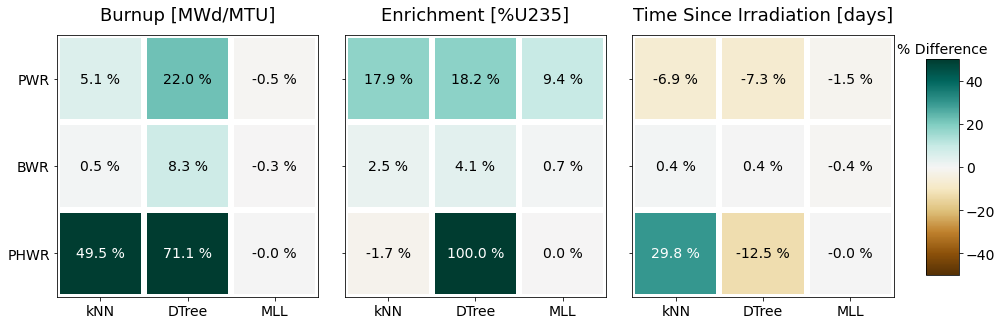
\includegraphics[width=\textwidth]{./chapters/exp1/rxtr-type_known-unknown_diff_err05.png}
  \caption[Heatmaps for three regression cases comparing known versus 
           unknown reactor type prior knowledge]
          {Heatmaps for the three regression cases showing the percent 
           difference in prediction error between a known reactor type 
           and unknown reactor type using a 5\% training set error.}
  \todo[inline]{would this be better shown with a plot that has little arrows? or leave like this?}
  \label{fig:knownrxtr}
\end{figure}

For burnup prediction, most differences are within $\pm10\%$ except for three
scenarios.  The decision tree algorithm has improved burnup prediction for
\gls{PWR}s by 22.0\% and for \gls{PHWR}s by 71.1\% given a known reactor type.
The \textit{k}-nearest neighbors algorithm has 49.5\% improved burnup
prediction for the \gls{PHWR}. For \gls{U235} enrichment, the \gls{PWR}
predictions improve by approximately 18\% for the scikit-learn algorithms.
Even though the value is within $\pm10\%$, this is the only scenario where
there is an appreciable difference in \gls{MLL} performance. The decision tree
enrichment prediction of \gls{PHWR}s also has a sizeable improvement of
100.0\%.  The time since irradiation predictions for the most part do not show
improvement outside of $\pm10\%$. Of note is some volatile behavior for the
\gls{PHWR} case with the scikit-learn algorithms.  While \textit{k}-nearest
neighbors improves by 29.8\%, the decision tree predictions were worse by
12.5\%.  Since the main concern here is showing how prediction performance
improves with prior reactor type knowledge, this reduction in performance is
odd but not worthy of further investigation.

The improvements in the \gls{PHWR} predictions are not surprising since the
generalization of the scikit-learn algorithms could lead to the unique
\gls{PHWR} cases being ignored, since they are after all only 1.5\% of the
training set.  Another interesting result is that the \gls{BWR} predictions
experience no large changes, which makes sense given that they comprise 72\% of
the training set. Also, the \gls{MLL} predictions are approximately the same,
which is expected because this algorithm does not generalize, and the
prediction comes as a set of labels and is therefore already linked to the
reactor type. Overall, it is important to be aware that the regression labels
coming from a \gls{PHWR} will be unlikely to be optimal results (except for
those from \gls{MLL} calculations).

%\begin{table}[!htb]
%  \centering
%  \begin{tabular}{@{}llllllll@{}}
%    \toprule
%    &  &  \multicolumn{2}{c}{\textit{k}NN} 
%    &     \multicolumn{2}{c}{Dec Trees} 
%    &     \multicolumn{2}{c}{MLL Calcs} \\ 
%    \toprule
%    \begin{tabular}[c]{@{}l@{}}Prediction\\ Parameter\end{tabular} &
%    \begin{tabular}[c]{@{}l@{}}Reactor \\ Type\end{tabular} &
%    K & U &  K & U & K & U \\ \midrule
%    \multirow{3}{*}{\begin{tabular}[c]{@{}l@{}}Burnup \\ \% {$[MWd/MTU]$} \end{tabular}}
%     & PWR  & 0.08  & 0.08  & 0.03 & 0.04 & 0.24 & 0.25 \\ 
%     & BWR  & 0.11  & 0.10  & 0.03 & 0.03 & 0.40 & 0.40 \\ 
%     & PHWR & 0.13  & 0.19  & 0.01 & 0.03 & 0.29 & 0.29 \\ \hline
%    \multirow{3}{*}{\begin{tabular}[c]{@{}l@{}}Enrichment \\ \% {$[\%\:{}^{235}\text{U}]$} \end{tabular}}
%     & PWR  & 0.10  & 0.11  & 0.02 & 0.02 & 0.26 & 0.29 \\ 
%     & BWR  & 0.12  & 0.12  & 0.02 & 0.02 & 0.46 & 0.46 \\ 
%     & PHWR & 0.00  & 0.00  & 0.00 & 0.00 & 0.00 & 0.00 \\ \hline
%    \multirow{3}{*}{\begin{tabular}[c]{@{}l@{}}Time Since \\ Irradiation \\ \% {$[days]$} \end{tabular}}
%     & PWR  & 6.47  & 6.13  & 1.50 & 1.43 & 1.55 & 1.46 \\ 
%     & BWR  & 9.18  & 9.15  & 1.56 & 1.53 & 2.07 & 2.05 \\ 
%     & PHWR & 13.78 & 18.62 & 4.51 & 3.71 & 2.30 & 2.30 \\ \bottomrule
%  \end{tabular}
%  \caption{\gls{MAPE}s for the three prediction cases for each algorithm at 1\% 
%           training set error. \textit{K} refers to \textit{known} reactor 
%           type and \textit{U} refers to \textit{unknown} reactor type prior 
%           to regression.}
%  \label{tbl:knownrxtr}
%\end{table}

%\begin{figure}[!htb]
%  \centering
%  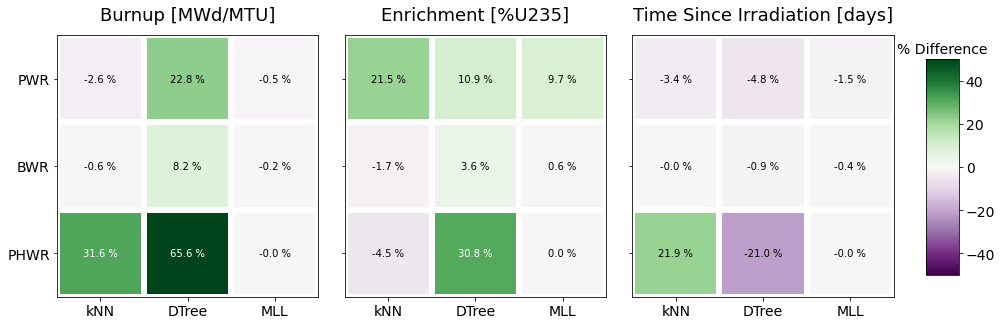
\includegraphics[width=\textwidth]{./chapters/exp1/rxtr-type_known-unknown_diff_err01.png}
%  \caption{Heatmaps for the three regression cases showing the percent 
%           difference in prediction error between a known reactor type 
%           and unknown reactor type.}
%  \label{fig:knownrxtr}
%\end{figure}

